\fullWidthTwoColumnFigureTable%
	[t] % Placement
	{0d/figures/sc_iii_uv_initial_condition.pdf} % Figure
	{fig:sc_iii_uv_initial_condition} % Figure label
	{%
		\uv{} potential $U ( \sigma )$ (red-dashed) and its first derivative $u ( \sigma ) = \partial_\sigma U ( \sigma )$ (blue, solid) of test case III from \cref{eq:testing_scenario_phi6}. 
		\fromFig{27}{zerod1}%
	} % Figure caption
	{%
		\renewcommand{\arraystretch}{1.15}
		\small
		\begin{tabular}{l c c c}
			\toprule
			$N$		&	$\Gamma^{(2)}$	&	$\Gamma^{(4)}$	&	$\Gamma^{(6)}$	\\
			\midrule
				$1$	&	$0.174051$	&	$0.015618$	&	$0.013440$\\
				$4$	&	$0.250333$	&	$0.048131$	&	$0.043282$\\
			\bottomrule
		\end{tabular}
	} % Table content
	{tab:sc_3_n_point_functions_exact}% Table label
	{%
		Exact results for $\Gamma^{(2n)}$ of the $O(N)$ model with the \uv{} initial potential \eqref{eq:testing_scenario_phi6} for selected $N$.
		They are obtained by a high-precision one-dimensional numerical integration of the expectation values $\langle ( \vec{\phi}^{\, 2} )^n \rangle$ from \cref{eq:ON_expectation_value} using \textit{NIntegrate} in \WAMXIIwR{}.
		Here, we present the first six digits only.
		\textit{In parts from Tab. III of \ccite{zerod1} and Tab. I of \ccite{zerod2}.}%
	} % Table caption
\subsubsection{Test case III: \texorpdfstring{$\phi^6$}{phi**6} potential}
\label{subsubsec:sc3}
For the third test case we consider the potential
\begin{align}
	U ( \vec{\varphi} \vts ) = \tfrac{1}{2} \, \vec{\varphi}^{\vts 2} - \tfrac{1}{20} \, ( \vec{\varphi}^{\vts 2} )^2 + \tfrac{1}{6!} \, ( \vec{\varphi}^{\vts 2} )^3\, .	\label{eq:testing_scenario_phi6}
\end{align}
This potential includes terms up to $( \vec{\varphi}^{\, 2} )^3$ and has two local minima and one local maximum and is therefore not convex.
The global minimum is located at $\vec{\varphi} = 0$ and the potential and its derivative (evaluated on the constant field configuration $\sigma$) are depicted in \cref{fig:sc_iii_uv_initial_condition}.
Selected reference values for the first three non-vanishing \nptFunctions{} can be found in \cref{tab:sc_3_n_point_functions_exact}.

We have again performed the full set of numerical tests of \cref{subsubsec:sc1} and found results supporting the general statements made in that subsection.
For brevity, we will not repeat the complete discussion of that subsubsection but instead focus again on selected results.\bigskip

\Cref{fig:sc_iii_on_4_n_800_xmax_10_lambda_1e12_tir_60_rg_flow} shows the \frg{} flow with the initial condition \eqref{eq:testing_scenario_phi6} for the $O(4)$ model computed with the \ktScheme{} again using \textit{NDSolve} of \WAMXIIwR{} with \textit{PrecisionGoal} and \textit{AccuracyGoal} of 10 for the \frg{} time evolution.
Both non-trivial local extrema fade away during \frg{} time evolution towards the \ir{}.
At $t \approx 28$ the potential $U ( t, \sigma )$ becomes convex as $u ( t, \sigma )$ turns strictly positive for $\sigma > 0$.
We again observe that the linear extrapolation used at the right boundary $x_\mathrm{max}$ of the computational domain seems surprisingly efficient even for an initial condition with quintic asymptotics.
Studying \cref{fig:sc_iii_on_4_deltax_25e-3_lambda_1e12_tir_60_errors_xmax} we observe that the relative errors in the \ir{} become independent of the size of the computational domain for $x_\mathrm{max}\smallergtrsim 6$.

\fullWidthTwoColumnFigures%
	[!t] % Placement
	{%
		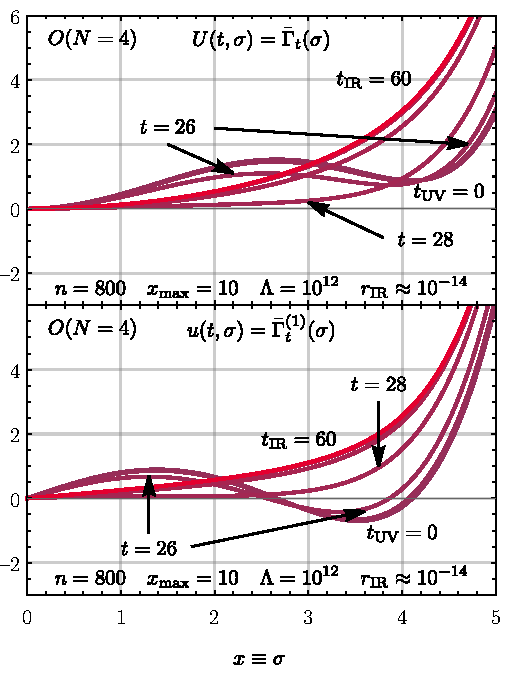
\includegraphics[width=\subcaptionFigureWidth]{0d/figures/sc_iii_on_4_n_800_xmax_10_lambda_1e12_tir_60_rg_flow.pdf} % left figure
		\captionsetup{width=\subcaptionFigureWidth}%
		\caption{
			The \frg{} flow of the effective potential $U ( t, \sigma )$ (upper panel) and its derivative $u ( t , \sigma ) = \partial_\sigma U ( t , \sigma )$ (lower panel) for the zero-dimensional $O ( 4 )$ model with initial condition \cref{eq:testing_scenario_phi6}, evaluated at $t = 0, \, 2, \, 4, \, \ldots, \, 60$ (integer values for $t$ were chosen for convenience and readability). 
			The (overlapping) {blue} and {violet} curves correspond to the \uv{} and the {red} curves to the \ir{}.
			We used the exponential regulator~\eqref{eq:exponential_regulator} with \uv{} scale $\Lambda = 10^{12}$.
			The plot does not show the region ${x \in[5,10]}$, because the tiny differences between $u ( t, \sigma )$ and $u ( t_\mathrm{UV}, \sigma )$ are not visible in this region and vanish for large $x = \sigma$ anyhow.
			\fromFig{28}{zerod1}
		}
		\label{fig:sc_iii_on_4_n_800_xmax_10_lambda_1e12_tir_60_rg_flow}%
	}
	{\fullWidthTwoColumnFigureSpacing}
	{
		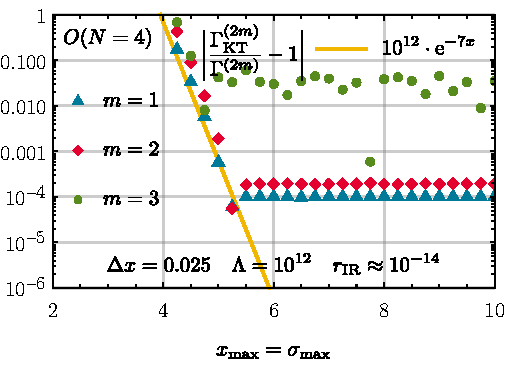
\includegraphics[width=\subcaptionFigureWidth]{0d/figures/sc_iii_on_4_deltax_25e-3_lambda_1e12_tir_60_errors_xmax.pdf} % Right figure
		\captionsetup{width=\subcaptionFigureWidth}%
		\caption{%
			The relative error for $\Gamma^{(2m)}$ for $m = 1, 2, 3$, for the $O ( 4 )$ model using the \uv{} potential \eqref{eq:testing_scenario_phi6}, as a function of the size of the computational interval $x_\mathrm{max}$. The cell size is $\Delta x = 0.025$. $\Gamma^{(2m)}$ are computed from the discrete values of the derivative of the \ir{} potential $u ( t_\mathrm{IR} = 60, \sigma )$ via the second-order accurate central finite-difference stencils \eqref{eq:derivative_1_central_error_2}, \eqref{eq:derivative_3_central_error_2}, and \eqref{eq:derivative_5_central_error_2} at $\sigma = 0$.
			We used the exponential regulator~\eqref{eq:exponential_regulator} with \uv{} scale $\Lambda = 10^{12}$.
			The yellow straight line $\propto\exp\del{-7\,x_\mathrm{max}}$ is for optical guidance.
			\fromFig{29}{zerod1}%
		}%
		\label{fig:sc_iii_on_4_deltax_25e-3_lambda_1e12_tir_60_errors_xmax}%
	}
\paragraph{\frg{} Taylor expansion: Concluding remarks}\phantomsection\label{paragraph:sc3taylorConclusion}\mbox{}\\
We were not able to evolve the \ode{} system of the Taylor expansion with the current initial condition to the \ir{} for any setup at all\footnote{%
	We thank J.~Eser for discussions on this issue and a cross-check using his \frg{} Taylor expansion code~\cite{Divotgey:2019xea,Cichutek:2020bli,Eser:2018jqo,Eser:2019pvd}, which reproduced our findings.
}. 
Independent of $n_\mathrm{trunc}$ and \ode{} integrator (\textit{NDSolve} of \WAMXIIwR{}) settings we encounter a numerical instability of the \ode{} systems at around $t \approx 28$ preventing a complete integration to the \ir{}.
The expansion coefficients $\bar{\Gamma}^{(2n)}(t)$ simply diverge at $t \approx 28$.
From \cref{fig:sc_iii_on_4_n_800_xmax_10_lambda_1e12_tir_60_rg_flow} we deduce that this is approximately the \rgtime{} point at which the non-trivial extrema vanish and the potential turns convex.
The precise underlying dynamics generated by the full \pde{} and resolved by the \ktScheme{} cannot be captured by the Taylor expansion (at least not in our set-up). 
However, also switching to a set-up with a $t$-dependent expansion point will not cure this problem, because the expansion point (the global minimum) does not move for this initial potential \dash{} a conscious design decision for test case III.
The instability of the solution of the coupled system of \odes{} might be explained \aposteriori{} by the formation of a non-analyticity at or around the \rgtime{} $t \approx 28$ of the collapse of the expansion.
Inevitably, due to the non-analyticity of the potential, Wilbraham-Gibbs-type~\cite{Wilbraham:1848,Gibbs:1898,Gibbs:1899} oscillations arise in the Taylor expansion, making the expansion scheme unstable~\cite{boyd2001chebyshev}.
This phenomenon is also observed and discussed in detail in the context of Fourier expansions of periodic potentials in the \frg{} in Sec.~2.2.2 of \ccite{Pangon:2010uf}.

However, a vertex expansion for a convex sextic potential including only positive coefficients in the \uv{} is possible, similar to $\phi^4$ theory with a positive mass term discussed at the end of the previous \cref{paragraph:sc2taylorPhiP}.
A numerical inversion of the \frg{} flow is again possible for systems with a small number of couplings.\bigskip

At this point we have discussed numerical results for the \frg{} Taylor expansion for quartic and sextic potentials.
The numerical performance in terms of achievable relative errors for the \nptFunctions{} in the \ir{} is rather poor for the quartic potential \eqref{eq:testing_scenario_phi4} with the negative mass term and very good for the potential with the positive mass term.
A numerical solution of \ode{} system of the Taylor expansion with the non-convex sextic potential \eqref{eq:testing_scenario_phi6} has proven impossible 

The zero-dimensional $O(N)$ model has proven very challenging for the Taylor expansion.
It seems that only convex, analytic \uv{} initial conditions and the resulting rather simple \frg{} flows can be treated with a vertex expansion in $\bar{\Gamma}^{(2n)}(t)$ around $\vec{\varphi} = 0$ in the zero-dimensional $O(N)$ model.

At this point we also want to reference our comments in \cref{sububsec:LAEBBE}: the treatment of non-linear advection-diffusion equations requires \apriori{} shock capturing schemes, capable of handling non-analyticities and even discontinuities.
An application of expansion schemes relying on analyticity like the Taylor expansion is only possible in very special situations and require an \aposteriori{} case-by-case evaluation of the method.
In scenarios where the \frg{} flows are driven by an interplay of advection and diffusion around non-trivial minima and/or large gradients of the conserved quantity $u$, the Taylor expansion is inevitably doomed to fail.
It is not possible to capture the dynamics of such equations reliably with the simple Taylor expansion discussed here.
A numerical inversion of the \grg{} flow is also impossible in those scenarios.
The appearance of a non-analytic behavior is also understood via a rise of entropy, \cf{} \cref{subsubsec:0dO1entResults,paragraph:infiniteNflowsEntropy}.

It should be noted that in this work we discussed the simplest possible Taylor/vertex-expansion scheme.
Other versions of the \frg{} Taylor (vertex) expansion including a moving expansion point or a rescaling of the expansion coefficients might improve the performance of the expansion scheme in certain cases, \cf{} \ccite{Litim:2002cf,Schaefer:2001cn,Rennecke:2015lur}.
Implementing and testing different approaches to the Taylor expansion for zero-dimensional $O(N)$ models would certainly be an interesting topic for further studies.